\documentclass[12pt]{article}
\usepackage[margin=1in]{geometry}
\usepackage{amsthm, amsmath, amsfonts, amssymb}
\usepackage{graphicx}
\usepackage[shortlabels]{enumitem}
\usepackage{setspace}
\usepackage{tcolorbox}
\usepackage[
  lambda,
  advantage,
  operators,
  adversary,
  landau,
  probability,
  sets,
  % notions,
  % logic,
  % ff,
  % mm,
  % primitives,
  % oracles,
  events,
  % complexity,
  asymptotics,
  keys,
]{cryptocode}
\doublespacing
\usepackage{hyperref}

\usepackage{pgfplots}
\pgfplotsset{compat=1.18}

\definecolor{cblueA}{HTML}{185FA5}
\definecolor{cblueB}{HTML}{378ADD}
\definecolor{cred}{HTML}{A32D2D}
\definecolor{ccoral}{HTML}{D85A30}
\definecolor{camber}{HTML}{BA7517}

%%% cryptocode tweaks
% Multi-letter variables, e.g., "ctr"
\NewDocumentCommand\var{m}{\ensuremath{\mathit{#1}}}
% Make keys and polynomials look like other identifiers.
% (No idea why cryptocode treats them specially.)
\RenewDocumentCommand\pckeystyle{m}{\ensuremath{\var{#1}}}
\RenewDocumentCommand\pcpolynomialstyle{m}{\ensuremath{\var{#1}}}
% Add 1pt padding to \gamechange (based on original definition).
\renewcommand{\gamechange}[2][gamechangecolor]{%
  {\setlength{\fboxsep}{1pt}%
    \colorbox{#1}{#2}}}
% Shorthand for \pcalgostyle
\NewDocumentCommand\algo{}{\pcalgostyle}
% Oracles
\NewDocumentCommand{\mathsc}{m}{{\normalfont\textsc{#1}}}
\RenewDocumentCommand\pcoraclestyle{m}{\ensuremath{\mathsc{#1}}}
\NewDocumentCommand\oracle{m}{\pcoraclestyle{#1}}
% Games
\newcommandx{\game}[4][3=\adv,4=(\secpar)]{{\operatorname{#1}_{#2}^{#3}#4}}
%\newcommand{\Game}{\algo{Game}}
% Misc
\newcommand{\pcsc}{\,;~}

\newcommand{\N}[0]{\mathbb{N}}
\newcommand{\Z}[0]{\mathbb{Z}}
\newcommand{\Q}[0]{\mathbb{Q}}
\newcommand{\F}[0]{\mathbb{F}}
\newcommand{\G}[0]{\mathbb{G}}
\newcommand{\pr}[1]{\text{Pr}\left[#1\right]}
\newcommand{\overarrow}[1]{\stackrel{#1}{\rightarrow}}
\newcommand{\verts}[1]{\left\vert #1\right\vert}
\newcommand{\M}{\mathcal{M}}
\newcommand{\C}{\mathcal{C}}
\newcommand{\K}{\mathcal{K}}
\newcommand{\Kpriv}{\mathcal{K}_{\text{priv}}}
\newcommand{\Kpub}{\mathcal{K}_{\text{pub}}}

\newtheorem{claim}{Claim}
\newtheorem{conj}{Conjecture}
\newtheorem{question}{Question}
\newtheorem{exercise}{Exercise}
\newtheorem{reading}{Reading}
\newtheorem{thm}[claim]{Theorem}
\newtheorem{lemma}[claim]{Lemma}
\newtheorem{prop}[claim]{Proposition}
\newtheorem{cor}[claim]{Corollary}
\theoremstyle{definition}
\newtheorem{definition}{Definition}

\theoremstyle{remark}
\newtheorem*{rem}{Remark}

\theoremstyle{definition}
\newtheorem{example}{Example}[section]


\begin{document}
\title{Week 3}
\author{Nadav Kohen}
\date{July 9, 2025}
\maketitle

This week has a little less content volume than last week, so I want to encourage you to also review and become more comfortable with the Week 2 documents and their exercises as part of this week's assignment.\\

Now that we have a little bit of experience working with security definitions using attack games and probabilities, our goal this week is to make all of the details rigorous to pave the way for the study of the security of Schnorr digital signatures, which we will continue next week.\\

The primary missing piece in our formalism from last week is the definition of the notion that a probability is ``negligible.'' Recall that this notion was central to all of our security definitions, which were all the result of requiring all advantage values to be negligible.

For those who like accompanying visuals, see Figure \ref{fig:negl}.\\
\begin{figure}
\begin{center}
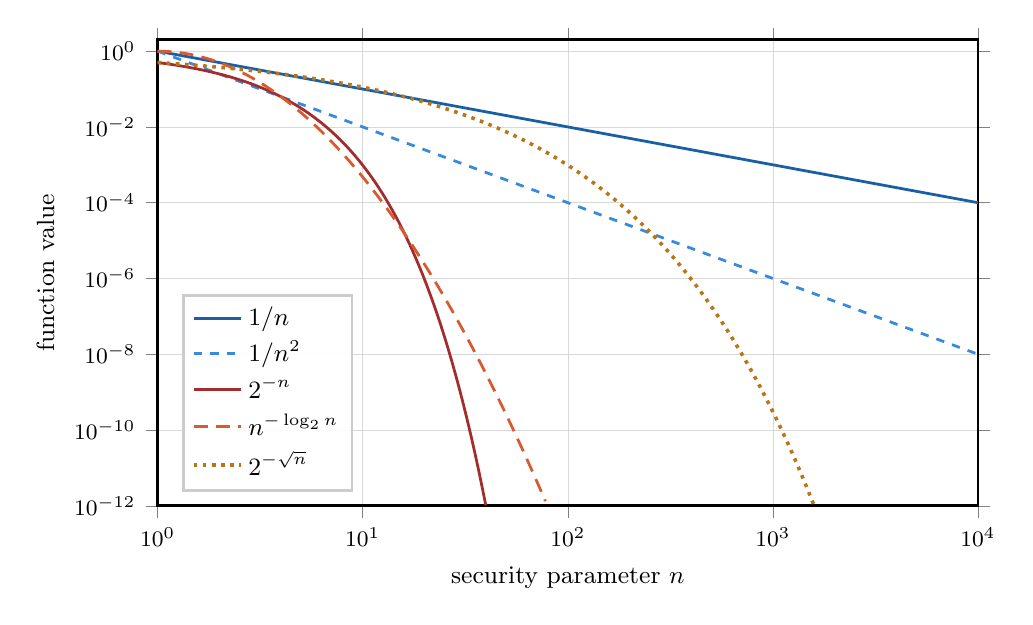
\begin{tikzpicture}
\begin{axis}[
    width=12cm, height=7.5cm,
    xmode=log, ymode=log,
    log basis x=10, log basis y=10,
    xlabel={security parameter $n$},
    ylabel={function value},
    xmin=1, xmax=10000,
    ymin=1e-12, ymax=2,
    xtick={1,10,100,1000,10000},
    ytick={1,1e-2,1e-4,1e-6,1e-8,1e-10,1e-12},
    grid=both,
    major grid style={line width=.2pt,draw=gray!30},
    minor grid style={draw=gray!12},
    tick align=outside,
    legend pos=south west,
    legend cell align={left},
    legend style={font=\small, draw=gray!40, fill=white, fill opacity=0.9, text opacity=1},
    label style={font=\small},
    tick label style={font=\footnotesize},
    line width=1pt,
]
 
\addplot[cblueA, solid] coordinates {(1,1.000000e+00) (1.04275,9.589991e-01) (1.08734,9.196792e-01) (1.13382,8.819715e-01) (1.1823,8.458098e-01) (1.23285,8.111308e-01) (1.28556,7.778737e-01) (1.34052,7.459802e-01) (1.39783,7.153943e-01) (1.45759,6.860624e-01) (1.51991,6.579332e-01) (1.58489,6.309573e-01) (1.65265,6.050875e-01) (1.72331,5.802783e-01) (1.79699,5.564864e-01) (1.87382,5.336699e-01) (1.95393,5.117890e-01) (2.03747,4.908051e-01) (2.12458,4.706817e-01) (2.21541,4.513833e-01) (2.31013,4.328761e-01) (2.4089,4.151278e-01) (2.51189,3.981072e-01) (2.61928,3.817844e-01) (2.73126,3.661309e-01) (2.84804,3.511192e-01) (2.9698,3.367230e-01) (3.09677,3.229170e-01) (3.22917,3.096771e-01) (3.36723,2.969800e-01) (3.51119,2.848036e-01) (3.66131,2.731264e-01) (3.81784,2.619279e-01) (3.98107,2.511886e-01) (4.15128,2.408897e-01) (4.32876,2.310130e-01) (4.51383,2.215412e-01) (4.70682,2.124578e-01) (4.90805,2.037469e-01) (5.11789,1.953930e-01) (5.3367,1.873817e-01) (5.56486,1.796989e-01) (5.80278,1.723311e-01) (6.05088,1.652654e-01) (6.30957,1.584893e-01) (6.57933,1.519911e-01) (6.86062,1.457593e-01) (7.15394,1.397831e-01) (7.4598,1.340518e-01) (7.77874,1.285556e-01) (8.11131,1.232847e-01) (8.4581,1.182299e-01) (8.81971,1.133824e-01) (9.19679,1.087336e-01) (9.58999,1.042754e-01) (10,1.000000e-01) (10.4275,9.589991e-02) (10.8734,9.196792e-02) (11.3382,8.819715e-02) (11.823,8.458098e-02) (12.3285,8.111308e-02) (12.8556,7.778737e-02) (13.4052,7.459802e-02) (13.9783,7.153943e-02) (14.5759,6.860624e-02) (15.1991,6.579332e-02) (15.8489,6.309573e-02) (16.5265,6.050875e-02) (17.2331,5.802783e-02) (17.9699,5.564864e-02) (18.7382,5.336699e-02) (19.5393,5.117890e-02) (20.3747,4.908051e-02) (21.2458,4.706817e-02) (22.1541,4.513833e-02) (23.1013,4.328761e-02) (24.089,4.151278e-02) (25.1189,3.981072e-02) (26.1928,3.817844e-02) (27.3126,3.661309e-02) (28.4804,3.511192e-02) (29.698,3.367230e-02) (30.9677,3.229170e-02) (32.2917,3.096771e-02) (33.6723,2.969800e-02) (35.1119,2.848036e-02) (36.6131,2.731264e-02) (38.1784,2.619279e-02) (39.8107,2.511886e-02) (41.5128,2.408897e-02) (43.2876,2.310130e-02) (45.1383,2.215412e-02) (47.0682,2.124578e-02) (49.0805,2.037469e-02) (51.1789,1.953930e-02) (53.367,1.873817e-02) (55.6486,1.796989e-02) (58.0278,1.723311e-02) (60.5088,1.652654e-02) (63.0957,1.584893e-02) (65.7933,1.519911e-02) (68.6062,1.457593e-02) (71.5394,1.397831e-02) (74.598,1.340518e-02) (77.7874,1.285556e-02) (81.1131,1.232847e-02) (84.581,1.182299e-02) (88.1971,1.133824e-02) (91.9679,1.087336e-02) (95.8999,1.042754e-02) (100,1.000000e-02) (104.275,9.589991e-03) (108.734,9.196792e-03) (113.382,8.819715e-03) (118.23,8.458098e-03) (123.285,8.111308e-03) (128.556,7.778737e-03) (134.052,7.459802e-03) (139.783,7.153943e-03) (145.759,6.860624e-03) (151.991,6.579332e-03) (158.489,6.309573e-03) (165.265,6.050875e-03) (172.331,5.802783e-03) (179.699,5.564864e-03) (187.382,5.336699e-03) (195.393,5.117890e-03) (203.747,4.908051e-03) (212.458,4.706817e-03) (221.541,4.513833e-03) (231.013,4.328761e-03) (240.89,4.151278e-03) (251.189,3.981072e-03) (261.928,3.817844e-03) (273.126,3.661309e-03) (284.804,3.511192e-03) (296.98,3.367230e-03) (309.677,3.229170e-03) (322.917,3.096771e-03) (336.723,2.969800e-03) (351.119,2.848036e-03) (366.131,2.731264e-03) (381.784,2.619279e-03) (398.107,2.511886e-03) (415.128,2.408897e-03) (432.876,2.310130e-03) (451.383,2.215412e-03) (470.682,2.124578e-03) (490.805,2.037469e-03) (511.789,1.953930e-03) (533.67,1.873817e-03) (556.486,1.796989e-03) (580.278,1.723311e-03) (605.088,1.652654e-03) (630.957,1.584893e-03) (657.933,1.519911e-03) (686.062,1.457593e-03) (715.394,1.397831e-03) (745.98,1.340518e-03) (777.874,1.285556e-03) (811.131,1.232847e-03) (845.81,1.182299e-03) (881.971,1.133824e-03) (919.679,1.087336e-03) (958.999,1.042754e-03) (1000,1.000000e-03) (1042.75,9.589991e-04) (1087.34,9.196792e-04) (1133.82,8.819715e-04) (1182.3,8.458098e-04) (1232.85,8.111308e-04) (1285.56,7.778737e-04) (1340.52,7.459802e-04) (1397.83,7.153943e-04) (1457.59,6.860624e-04) (1519.91,6.579332e-04) (1584.89,6.309573e-04) (1652.65,6.050875e-04) (1723.31,5.802783e-04) (1796.99,5.564864e-04) (1873.82,5.336699e-04) (1953.93,5.117890e-04) (2037.47,4.908051e-04) (2124.58,4.706817e-04) (2215.41,4.513833e-04) (2310.13,4.328761e-04) (2408.9,4.151278e-04) (2511.89,3.981072e-04) (2619.28,3.817844e-04) (2731.26,3.661309e-04) (2848.04,3.511192e-04) (2969.8,3.367230e-04) (3096.77,3.229170e-04) (3229.17,3.096771e-04) (3367.23,2.969800e-04) (3511.19,2.848036e-04) (3661.31,2.731264e-04) (3817.84,2.619279e-04) (3981.07,2.511886e-04) (4151.28,2.408897e-04) (4328.76,2.310130e-04) (4513.83,2.215412e-04) (4706.82,2.124578e-04) (4908.05,2.037469e-04) (5117.89,1.953930e-04) (5336.7,1.873817e-04) (5564.86,1.796989e-04) (5802.78,1.723311e-04) (6050.88,1.652654e-04) (6309.57,1.584893e-04) (6579.33,1.519911e-04) (6860.62,1.457593e-04) (7153.94,1.397831e-04) (7459.8,1.340518e-04) (7778.74,1.285556e-04) (8111.31,1.232847e-04) (8458.1,1.182299e-04) (8819.71,1.133824e-04) (9196.79,1.087336e-04) (9589.99,1.042754e-04) (10000,1.000000e-04)};
\addlegendentry{$1/n$}
 
\addplot[cblueB, dashed] coordinates {(1,1.000000e+00) (1.04275,9.196792e-01) (1.08734,8.458098e-01) (1.13382,7.778737e-01) (1.1823,7.153943e-01) (1.23285,6.579332e-01) (1.28556,6.050875e-01) (1.34052,5.564864e-01) (1.39783,5.117890e-01) (1.45759,4.706817e-01) (1.51991,4.328761e-01) (1.58489,3.981072e-01) (1.65265,3.661309e-01) (1.72331,3.367230e-01) (1.79699,3.096771e-01) (1.87382,2.848036e-01) (1.95393,2.619279e-01) (2.03747,2.408897e-01) (2.12458,2.215412e-01) (2.21541,2.037469e-01) (2.31013,1.873817e-01) (2.4089,1.723311e-01) (2.51189,1.584893e-01) (2.61928,1.457593e-01) (2.73126,1.340518e-01) (2.84804,1.232847e-01) (2.9698,1.133824e-01) (3.09677,1.042754e-01) (3.22917,9.589991e-02) (3.36723,8.819715e-02) (3.51119,8.111308e-02) (3.66131,7.459802e-02) (3.81784,6.860624e-02) (3.98107,6.309573e-02) (4.15128,5.802783e-02) (4.32876,5.336699e-02) (4.51383,4.908051e-02) (4.70682,4.513833e-02) (4.90805,4.151278e-02) (5.11789,3.817844e-02) (5.3367,3.511192e-02) (5.56486,3.229170e-02) (5.80278,2.969800e-02) (6.05088,2.731264e-02) (6.30957,2.511886e-02) (6.57933,2.310130e-02) (6.86062,2.124578e-02) (7.15394,1.953930e-02) (7.4598,1.796989e-02) (7.77874,1.652654e-02) (8.11131,1.519911e-02) (8.4581,1.397831e-02) (8.81971,1.285556e-02) (9.19679,1.182299e-02) (9.58999,1.087336e-02) (10,1.000000e-02) (10.4275,9.196792e-03) (10.8734,8.458098e-03) (11.3382,7.778737e-03) (11.823,7.153943e-03) (12.3285,6.579332e-03) (12.8556,6.050875e-03) (13.4052,5.564864e-03) (13.9783,5.117890e-03) (14.5759,4.706817e-03) (15.1991,4.328761e-03) (15.8489,3.981072e-03) (16.5265,3.661309e-03) (17.2331,3.367230e-03) (17.9699,3.096771e-03) (18.7382,2.848036e-03) (19.5393,2.619279e-03) (20.3747,2.408897e-03) (21.2458,2.215412e-03) (22.1541,2.037469e-03) (23.1013,1.873817e-03) (24.089,1.723311e-03) (25.1189,1.584893e-03) (26.1928,1.457593e-03) (27.3126,1.340518e-03) (28.4804,1.232847e-03) (29.698,1.133824e-03) (30.9677,1.042754e-03) (32.2917,9.589991e-04) (33.6723,8.819715e-04) (35.1119,8.111308e-04) (36.6131,7.459802e-04) (38.1784,6.860624e-04) (39.8107,6.309573e-04) (41.5128,5.802783e-04) (43.2876,5.336699e-04) (45.1383,4.908051e-04) (47.0682,4.513833e-04) (49.0805,4.151278e-04) (51.1789,3.817844e-04) (53.367,3.511192e-04) (55.6486,3.229170e-04) (58.0278,2.969800e-04) (60.5088,2.731264e-04) (63.0957,2.511886e-04) (65.7933,2.310130e-04) (68.6062,2.124578e-04) (71.5394,1.953930e-04) (74.598,1.796989e-04) (77.7874,1.652654e-04) (81.1131,1.519911e-04) (84.581,1.397831e-04) (88.1971,1.285556e-04) (91.9679,1.182299e-04) (95.8999,1.087336e-04) (100,1.000000e-04) (104.275,9.196792e-05) (108.734,8.458098e-05) (113.382,7.778737e-05) (118.23,7.153943e-05) (123.285,6.579332e-05) (128.556,6.050875e-05) (134.052,5.564864e-05) (139.783,5.117890e-05) (145.759,4.706817e-05) (151.991,4.328761e-05) (158.489,3.981072e-05) (165.265,3.661309e-05) (172.331,3.367230e-05) (179.699,3.096771e-05) (187.382,2.848036e-05) (195.393,2.619279e-05) (203.747,2.408897e-05) (212.458,2.215412e-05) (221.541,2.037469e-05) (231.013,1.873817e-05) (240.89,1.723311e-05) (251.189,1.584893e-05) (261.928,1.457593e-05) (273.126,1.340518e-05) (284.804,1.232847e-05) (296.98,1.133824e-05) (309.677,1.042754e-05) (322.917,9.589991e-06) (336.723,8.819715e-06) (351.119,8.111308e-06) (366.131,7.459802e-06) (381.784,6.860624e-06) (398.107,6.309573e-06) (415.128,5.802783e-06) (432.876,5.336699e-06) (451.383,4.908051e-06) (470.682,4.513833e-06) (490.805,4.151278e-06) (511.789,3.817844e-06) (533.67,3.511192e-06) (556.486,3.229170e-06) (580.278,2.969800e-06) (605.088,2.731264e-06) (630.957,2.511886e-06) (657.933,2.310130e-06) (686.062,2.124578e-06) (715.394,1.953930e-06) (745.98,1.796989e-06) (777.874,1.652654e-06) (811.131,1.519911e-06) (845.81,1.397831e-06) (881.971,1.285556e-06) (919.679,1.182299e-06) (958.999,1.087336e-06) (1000,1.000000e-06) (1042.75,9.196792e-07) (1087.34,8.458098e-07) (1133.82,7.778737e-07) (1182.3,7.153943e-07) (1232.85,6.579332e-07) (1285.56,6.050875e-07) (1340.52,5.564864e-07) (1397.83,5.117890e-07) (1457.59,4.706817e-07) (1519.91,4.328761e-07) (1584.89,3.981072e-07) (1652.65,3.661309e-07) (1723.31,3.367230e-07) (1796.99,3.096771e-07) (1873.82,2.848036e-07) (1953.93,2.619279e-07) (2037.47,2.408897e-07) (2124.58,2.215412e-07) (2215.41,2.037469e-07) (2310.13,1.873817e-07) (2408.9,1.723311e-07) (2511.89,1.584893e-07) (2619.28,1.457593e-07) (2731.26,1.340518e-07) (2848.04,1.232847e-07) (2969.8,1.133824e-07) (3096.77,1.042754e-07) (3229.17,9.589991e-08) (3367.23,8.819715e-08) (3511.19,8.111308e-08) (3661.31,7.459802e-08) (3817.84,6.860624e-08) (3981.07,6.309573e-08) (4151.28,5.802783e-08) (4328.76,5.336699e-08) (4513.83,4.908051e-08) (4706.82,4.513833e-08) (4908.05,4.151278e-08) (5117.89,3.817844e-08) (5336.7,3.511192e-08) (5564.86,3.229170e-08) (5802.78,2.969800e-08) (6050.88,2.731264e-08) (6309.57,2.511886e-08) (6579.33,2.310130e-08) (6860.62,2.124578e-08) (7153.94,1.953930e-08) (7459.8,1.796989e-08) (7778.74,1.652654e-08) (8111.31,1.519911e-08) (8458.1,1.397831e-08) (8819.71,1.285556e-08) (9196.79,1.182299e-08) (9589.99,1.087336e-08) (10000,1.000000e-08)};
\addlegendentry{$1/n^2$}
 
\addplot[cred, solid] coordinates {(1,5.000000e-01) (1.04275,4.854000e-01) (1.08734,4.706297e-01) (1.13382,4.557064e-01) (1.1823,4.406488e-01) (1.23285,4.254771e-01) (1.28556,4.102128e-01) (1.34052,3.948788e-01) (1.39783,3.794994e-01) (1.45759,3.641000e-01) (1.51991,3.487074e-01) (1.58489,3.333493e-01) (1.65265,3.180546e-01) (1.72331,3.028529e-01) (1.79699,2.877745e-01) (1.87382,2.728505e-01) (1.95393,2.581121e-01) (2.03747,2.435908e-01) (2.12458,2.293180e-01) (2.21541,2.153250e-01) (2.31013,2.016423e-01) (2.4089,1.882998e-01) (2.51189,1.753262e-01) (2.61928,1.627490e-01) (2.73126,1.505940e-01) (2.84804,1.388851e-01) (2.9698,1.276442e-01) (3.09677,1.168905e-01) (3.22917,1.066407e-01) (3.36723,9.690873e-02) (3.51119,8.770533e-02) (3.66131,7.903805e-02) (3.81784,7.091113e-02) (3.98107,6.332541e-02) (4.15128,5.627828e-02) (4.32876,4.976374e-02) (4.51383,4.377246e-02) (4.70682,3.829191e-02) (4.90805,3.330653e-02) (5.11789,2.879796e-02) (5.3367,2.474534e-02) (5.56486,2.112560e-02) (5.80278,1.791382e-02) (6.05088,1.508360e-02) (6.30957,1.260750e-02) (6.57933,1.045740e-02) (6.86062,8.604909e-03) (7.15394,7.021804e-03) (7.4598,5.680362e-03) (7.77874,4.553725e-03) (8.11131,3.616204e-03) (8.4581,2.843536e-03) (8.81971,2.213101e-03) (9.19679,1.704079e-03) (9.58999,1.297553e-03) (10,9.765625e-04) (10.4275,7.261026e-04) (10.8734,5.330813e-04) (11.3382,3.862346e-04) (11.823,2.760106e-04) (12.3285,1.944292e-04) (12.8556,1.349248e-04) (13.4052,9.218028e-05) (13.9783,6.195988e-05) (14.5759,4.094557e-05) (15.1991,2.658347e-05) (15.8489,1.694323e-05) (16.5265,1.059295e-05) (17.2331,6.491084e-06) (17.9699,3.895145e-06) (18.7382,2.286902e-06) (19.5393,1.312452e-06) (20.3747,7.355439e-07) (21.2458,4.021446e-07) (22.1541,2.142618e-07) (23.1013,1.111263e-07) (24.089,5.604002e-08) (25.1189,2.744533e-08) (26.1928,1.303718e-08) (27.3126,5.998973e-09) (28.4804,2.670286e-09) (29.698,1.148179e-09) (30.9677,4.762011e-10) (32.2917,1.902084e-10) (33.6723,7.305147e-11) (35.1119,2.693145e-11) (36.6131,9.513979e-12) (38.1784,3.214728e-12) (39.8107,1.037003e-12)};
\addlegendentry{$2^{-n}$}
 
\addplot[ccoral, dash pattern=on 5pt off 3pt] coordinates {(1,1.000000e+00) (1.04275,9.974746e-01) (1.08734,9.899366e-01) (1.13382,9.774996e-01) (1.1823,9.603498e-01) (1.23285,9.387416e-01) (1.28556,9.129906e-01) (1.34052,8.834668e-01) (1.39783,8.505853e-01) (1.45759,8.147966e-01) (1.51991,7.765764e-01) (1.58489,7.364154e-01) (1.65265,6.948087e-01) (1.72331,6.522458e-01) (1.79699,6.092016e-01) (1.87382,5.661277e-01) (1.95393,5.234456e-01) (2.03747,4.815400e-01) (2.12458,4.407545e-01) (2.21541,4.013885e-01) (2.31013,3.636945e-01) (2.4089,3.278780e-01) (2.51189,2.940976e-01) (2.61928,2.624668e-01) (2.73126,2.330564e-01) (2.84804,2.058976e-01) (2.9698,1.809861e-01) (3.09677,1.582861e-01) (3.22917,1.377349e-01) (3.36723,1.192474e-01) (3.51119,1.027206e-01) (3.66131,8.803799e-02) (3.81784,7.507341e-02) (3.98107,6.369508e-02) (4.15128,5.376867e-02) (4.32876,4.516026e-02) (4.51383,3.773872e-02) (4.70682,3.137774e-02) (4.90805,2.595732e-02) (5.11789,2.136494e-02) (5.3367,1.749634e-02) (5.56486,1.425596e-02) (5.80278,1.155711e-02) (6.05088,9.321929e-03) (6.30957,7.481110e-03) (6.57933,5.973515e-03) (6.86062,4.745670e-03) (7.15394,3.751188e-03) (7.4598,2.950148e-03) (7.77874,2.308461e-03) (8.11131,1.797235e-03) (8.4581,1.392166e-03) (8.81971,1.072953e-03) (9.19679,8.227617e-04) (9.58999,6.277275e-04) (10,4.765099e-04) (10.4275,3.598955e-04) (10.8734,2.704485e-04) (11.3382,2.022071e-04) (11.823,1.504222e-04) (12.3285,1.113348e-04) (12.8556,8.198868e-05) (13.4052,6.007316e-05) (13.9783,4.379361e-05) (14.5759,3.176469e-05) (15.1991,2.292357e-05) (15.8489,1.645976e-05) (16.5265,1.175895e-05) (17.2331,8.358285e-06) (17.9699,5.911117e-06) (18.7382,4.159351e-06) (19.5393,2.911959e-06) (20.3747,2.028377e-06) (21.2458,1.405775e-06) (22.1541,9.693632e-07) (23.1013,6.650602e-07) (24.089,4.539825e-07) (25.1189,3.083337e-07) (26.1928,2.083562e-07) (27.3126,1.400863e-07) (28.4804,9.371055e-08) (29.698,6.237134e-08) (30.9677,4.130335e-08) (32.2917,2.721380e-08) (33.6723,1.784008e-08) (35.1119,1.163612e-08) (36.6131,7.551324e-09) (38.1784,4.875753e-09) (39.8107,3.132305e-09) (41.5128,2.002120e-09) (43.2876,1.273268e-09) (45.1383,8.056626e-10) (47.0682,5.072129e-10) (49.0805,3.177101e-10) (51.1789,1.980047e-10) (53.367,1.227789e-10) (55.6486,7.574874e-11) (58.0278,4.649764e-11) (60.5088,2.839815e-11) (63.0957,1.725651e-11) (65.7933,1.043325e-11) (68.6062,6.276099e-12) (71.5394,3.756329e-12) (74.598,2.236873e-12) (77.7874,1.325325e-12)};
\addlegendentry{$n^{-\log_2 n}$}
 
\addplot[camber, dotted, line width=1.3pt] coordinates {(1,5.000000e-01) (1.04275,4.927223e-01) (1.08734,4.854000e-01) (1.13382,4.780351e-01) (1.1823,4.706297e-01) (1.23285,4.631860e-01) (1.28556,4.557064e-01) (1.34052,4.481931e-01) (1.39783,4.406488e-01) (1.45759,4.330759e-01) (1.51991,4.254771e-01) (1.58489,4.178551e-01) (1.65265,4.102128e-01) (1.72331,4.025530e-01) (1.79699,3.948788e-01) (1.87382,3.871932e-01) (1.95393,3.794994e-01) (2.03747,3.718005e-01) (2.12458,3.641000e-01) (2.21541,3.564012e-01) (2.31013,3.487074e-01) (2.4089,3.410223e-01) (2.51189,3.333493e-01) (2.61928,3.256922e-01) (2.73126,3.180546e-01) (2.84804,3.104402e-01) (2.9698,3.028529e-01) (3.09677,2.952964e-01) (3.22917,2.877745e-01) (3.36723,2.802913e-01) (3.51119,2.728505e-01) (3.66131,2.654561e-01) (3.81784,2.581121e-01) (3.98107,2.508223e-01) (4.15128,2.435908e-01) (4.32876,2.364214e-01) (4.51383,2.293180e-01) (4.70682,2.222846e-01) (4.90805,2.153250e-01) (5.11789,2.084430e-01) (5.3367,2.016423e-01) (5.56486,1.949267e-01) (5.80278,1.882998e-01) (6.05088,1.817651e-01) (6.30957,1.753262e-01) (6.57933,1.689864e-01) (6.86062,1.627490e-01) (7.15394,1.566172e-01) (7.4598,1.505940e-01) (7.77874,1.446824e-01) (8.11131,1.388851e-01) (8.4581,1.332049e-01) (8.81971,1.276442e-01) (9.19679,1.222053e-01) (9.58999,1.168905e-01) (10,1.117016e-01) (10.4275,1.066407e-01) (10.8734,1.017092e-01) (11.3382,9.690873e-02) (11.823,9.224041e-02) (12.3285,8.770533e-02) (12.8556,8.330433e-02) (13.4052,7.903805e-02) (13.9783,7.490691e-02) (14.5759,7.091113e-02) (15.1991,6.705070e-02) (15.8489,6.332541e-02) (16.5265,5.973482e-02) (17.2331,5.627828e-02) (17.9699,5.295494e-02) (18.7382,4.976374e-02) (19.5393,4.670340e-02) (20.3747,4.377246e-02) (21.2458,4.096925e-02) (22.1541,3.829191e-02) (23.1013,3.573841e-02) (24.089,3.330653e-02) (25.1189,3.099389e-02) (26.1928,2.879796e-02) (27.3126,2.671605e-02) (28.4804,2.474534e-02) (29.698,2.288288e-02) (30.9677,2.112560e-02) (32.2917,1.947033e-02) (33.6723,1.791382e-02) (35.1119,1.645271e-02) (36.6131,1.508360e-02) (38.1784,1.380304e-02) (39.8107,1.260750e-02) (41.5128,1.149347e-02) (43.2876,1.045740e-02) (45.1383,9.495724e-03) (47.0682,8.604909e-03) (49.0805,7.781432e-03) (51.1789,7.021804e-03) (53.367,6.322577e-03) (55.6486,5.680362e-03) (58.0278,5.091829e-03) (60.5088,4.553725e-03) (63.0957,4.062878e-03) (65.7933,3.616204e-03) (68.6062,3.210717e-03) (71.5394,2.843536e-03) (74.598,2.511884e-03) (77.7874,2.213101e-03) (81.1131,1.944641e-03) (84.581,1.704079e-03) (88.1971,1.489110e-03) (91.9679,1.297553e-03) (95.8999,1.127349e-03) (100,9.765625e-04) (104.275,8.433785e-04) (108.734,7.261026e-04) (113.382,6.231578e-04) (118.23,5.330813e-04) (123.285,4.545217e-04) (128.556,3.862346e-04) (134.052,3.270786e-04) (139.783,2.760106e-04) (145.759,2.320812e-04) (151.991,1.944292e-04) (158.489,1.622770e-04) (165.265,1.349248e-04) (172.331,1.117457e-04) (179.699,9.218028e-05) (187.382,7.573160e-05) (195.393,6.195988e-05) (203.747,5.047777e-05) (212.458,4.094557e-05) (221.541,3.306671e-05) (231.013,2.658347e-05) (240.89,2.127294e-05) (251.189,1.694323e-05) (261.928,1.342994e-05) (273.126,1.059295e-05) (284.804,8.313430e-06) (296.98,6.491084e-06) (309.677,5.041747e-06) (322.917,3.895145e-06) (336.723,2.992925e-06) (351.119,2.286902e-06) (366.131,1.737511e-06) (381.784,1.312452e-06) (398.107,9.855121e-07) (415.128,7.355439e-07) (432.876,5.455915e-07) (451.383,4.021446e-07) (470.682,2.945061e-07) (490.805,2.142618e-07) (511.789,1.548363e-07) (533.67,1.111263e-07) (556.486,7.919784e-08) (580.278,5.604002e-08) (605.088,3.936459e-08) (630.957,2.744533e-08) (657.933,1.898968e-08) (686.062,1.303718e-08) (715.394,8.879618e-09) (745.98,5.998973e-09) (777.874,4.019359e-09) (811.131,2.670286e-09) (845.81,1.758741e-09) (881.971,1.148179e-09) (919.679,7.428484e-10) (958.999,4.762011e-10) (1000,3.024097e-10) (1042.75,1.902084e-10) (1087.34,1.184688e-10) (1133.82,7.305147e-11) (1182.3,4.458740e-11) (1232.85,2.693145e-11) (1285.56,1.609443e-11) (1340.52,9.513979e-12) (1397.83,5.561848e-12) (1457.59,3.214728e-12) (1519.91,1.836680e-12) (1584.89,1.037003e-12)};
\addlegendentry{$2^{-\sqrt{n}}$}
 
\end{axis}
\end{tikzpicture}
\end{center}
\caption{A negligible function eventually dips below every inverse polynomial, no matter how large its degree. On a log-log plot like the one above, the inverse polynomials $\frac{1}{n^c}$ are straight lines (with slope -c); a negligible function is a curve that eventually bends away from all such lines. Read the picture as a race to the bottom. The two blue lines are non-negligible reference functions -- they decay, but only at a polynomial rate. Each warm curve is negligible, and each eventually undercuts every blue line.}\label{fig:negl}
\end{figure}

\begin{reading}\label{negl}
Read about negligible functions and probabilities in:\\
Mike Rosulek - The Joy of Cryptography - pages 67-71.
\end{reading}

In Reading \ref{negl}, we encountered the following two equivalent definitions of what it means for a function, $f$, to be negligible:
\begin{itemize}
\item For all polynomials, $p$, $\lim_{\lambda\to\infty}p(\lambda)\cdot f(\lambda) = 0$.
\item For all natural numbers, $c$, $\lim_{\lambda\to\infty}\lambda^c\cdot f(\lambda) = 0$.
\end{itemize}
The following are three additional equivalent definitions:
\begin{itemize}
\item For all polynomials, $p$, here exists a natural number, $N$, such that for all $\lambda>N$, $\verts{f(\lambda)}\leq \frac{1}{\verts{p(\lambda)}}$.
\item For all polynomials, $p$, here exists a natural number, $N$, such that for all $\lambda>N$, $\frac{1}{\verts{f(\lambda)}}\geq \verts{p(\lambda)}$.
\item For all natural numbers, $c$, here exists a natural number, $N$, such that for all $\lambda>N$, $\frac{1}{\verts{f(\lambda)}}\geq \verts{\lambda^c}$.
\end{itemize}
All three of these statements are more-or-less equivalent to the statement that $f$ grows smaller faster than the reciprocal of any polynomial, or equivalently that the reciprocal of $f$ grows larger faster than any polynomial. From this perspective, I hope that it is clear that the first two definitions from the reading are also capturing this idea. With this intuition in mind,

\begin{exercise}
Prove that a function, $f$ satisfying any one of the above properties satisfies all of the above properties. (Some of you may prefer to do some or all of Exercise 2 before Exercise 1, which is totally fine).
\end{exercise}

You may now use any of these definitions interchangeably as it suits you.

\begin{exercise}
The final page of Reading \ref{negl} has exercises demonstrating properties of negligible functions. Complete Exercises 4.2, 4.3(a), 4.3(b), 4.4 and 4.5.
\end{exercise}

\begin{exercise}
Now that we have some more comfort with the formal definition of negligible, double-check, for rigor, your solutions to Exercises 4 from 2a and 8 from last week (2b).
\end{exercise}

One last note on our formal model for cryptographic security proofs is the type of adversaries we allow. Namely, we do not allow the adversary to be an arbitrary program, but rather we require it to be a Probabalistic Polynomial Time (PPT) program. By ``Probabalistic,'' we mean that the adversary is allowed to use randomness, such as internal coin flips. By ``Polynomial Time,'' we mean that the number of steps in any execution of $\adv$ must be bounded by some polynomial, $p(\lambda)$. This assumption is not only sensical and practical, but it is also necessary for our definition of negligible to work because it ensures that our adversary cannot turn a negligible success probability into a non-negligible one by brute force (for example, the adversary may not sample a non-negligible proportion of all possible private keys).\\

Let us now begin our study of Schnorr signatures, beginning with the definition of security of a signature scheme: (keep in mind that an ``oracle'' in cryptography is simply a program that all other programs have access to as an interface that takes an input and returns an output, but no party has access to any information about the source code of this program beyond the specification; also note that a PPT adversary can make at most a polynomial-bounded number of queries to any oracle)

\begin{reading}
Read about the definition of Existentially UnForgable under Chosen Message Attack (EUF-CMA) in:\\
Jonathan Katz and Yehuda Lindell - Introduction to Modern Cryptography - pages 463-468.
\end{reading}

Note that when Katz and Lindell refer to $n$, they are talking about the security parameter, which we have been calling $\lambda$.\\

Before practicing with this definition, let us restate the book's definition in the attack-game notation we used last week, and then work through two examples --- one proving a scheme secure and one breaking a scheme --- since the exercise below will ask you to do both.\\

A (digital) signature scheme is a triple of PPT algorithms $(G, S, V)$: the key generation algorithm $G(\lambda)$ outputs a key pair $(pk, sk)$; the signing algorithm $S(sk, m)$ outputs a signature $\sigma$ on a message $m$; and the (deterministic) verification algorithm $V(pk, m, \sigma)$ outputs true or false. We require correctness: an honestly produced signature always verifies. The EUF-CMA attack game from the reading can then be written as the game $\game{\algo{EUF\text{-}CMA}}{}$ in Figure \ref{fig:eufcma}. The adversary is given the public key and access to a signing oracle $\oracle{Sign}$ (modeling the ``chosen message attack''), and it wins if it can produce a valid signature on \emph{any} message it did not already ask the oracle to sign (modeling ``existential forgery''). The set $Q$ simply records every message the adversary has queried, so that the final check $m^*\notin Q$ enforces that the forgery is on a fresh message.

\begin{figure}[tbhp]
  \begin{minipage}[t]{0.5\textwidth}\begin{flushright}
    \begin{tcolorbox}[width=6cm]
      \begin{pchstack}[center]
          \procedure[headlinesep=1pt]{$\game{\algo{EUF\text{-}CMA}}{}$}{%
            Q \gets \emptyset \\
            (pk, sk) \gets G(\lambda) \\
            (m^*, \sigma^*) \gets \adv^{\oracle{Sign}}(pk) \\
            \pcreturn V(pk, m^*, \sigma^*) \land m^*\notin Q
          }
      \end{pchstack}
    \end{tcolorbox}\end{flushright}\end{minipage}\begin{minipage}[t]{0.5\textwidth}
    \begin{tcolorbox}[width=5cm]
      \begin{pchstack}[center]
          \procedure[headlinesep=1pt]{$\oracle{Sign}(m)$}{%
            Q \gets Q\cup\{m\} \\
            \pcreturn S(sk, m)
          }
      \end{pchstack}
    \end{tcolorbox}
  \end{minipage}
  \caption{The EUF-CMA attack game for a signature scheme $(G,S,V)$. The adversary $\adv$ has oracle access to $\oracle{Sign}$, which signs any requested message and records it in $Q$; $\adv$ wins by outputting a valid signature on a message it never sent to $\oracle{Sign}$.\label{fig:eufcma}}
\end{figure}

As usual, we define the advantage of an adversary to be its probability of winning, $$\advantage{EUF\text{-}CMA}{\adv} := \pr{\game{\algo{EUF\text{-}CMA}}{} = \text{true}},$$ and we say that the signature scheme $(G, S, V)$ is secure (i.e., EUF-CMA secure) if $\advantage{EUF\text{-}CMA}{\adv}$ is negligible for every PPT adversary $\adv$. Notice that, unlike the distinguishing games from last week, here there is no ``$-\frac{1}{2}$'': a forger does not get to win half the time by guessing, since blindly outputting a signature on a fresh message succeeds only with negligible probability against a secure scheme.\\

\textbf{Example: proving security by reduction.} Suppose $(G, S, V)$ is an EUF-CMA secure signature scheme with message space $\{0,1\}^\lambda$. Consider the new scheme $(G, S', V')$ with message space $\{0,1\}^{\lambda-1}$ that signs a message after prepending a fixed $0$ bit: $$S'(sk, m) = S(sk, 0\,\|\,m), \qquad V'(pk, m, \sigma) = V(pk, 0\,\|\,m, \sigma),$$ where $\|$ denotes concatenation and key generation is unchanged. Intuitively, one would assume that $(G, S', V')$ is also EUF-CMA secure since adding this zero bit is inconsequential, but there are many situations in cryptography when seemingly inconsequential alterations do break the security of a protocol. As such, we will rigorously prove that this modification is secure if you started with a secure signature scheme, and of course we will prove this by reduction.\\

Following the recipe from Week 2a, the implication we want is ``($(G,S,V)$ is secure) $\Rightarrow$ ($(G,S',V')$ is secure),'' so we prove its contrapositive: we assume a PPT adversary $\adv$ that forges against $(G,S',V')$ with non-negligible advantage, and we build a PPT adversary $\adv'$ that forges against $(G,S,V)$ with non-negligible advantage. Our ``magic box'' is $\adv$; the new wrinkle, compared to the reductions of Week 2a, is that $\adv$ expects to interact with a signing oracle, so $\adv'$ must \emph{simulate that oracle} for $\adv$.\\

The reduction $\adv'$ is given $pk$ and access to the signing oracle $\oracle{Sign}(\cdot) = S(sk, \cdot)$ for the base scheme, and works as follows (see Figure \ref{fig:reduction} for the corresponding box-within-a-box diagram).
\begin{enumerate}[(1)]
\item Run $\adv(pk)$.
\item Whenever $\adv$ queries its signing oracle on a message $m \in \{0,1\}^{\lambda-1}$, answer it by querying our own oracle on $0\,\|\,m$ and returning the result $S(sk, 0\,\|\,m)$. Since this equals $S'(sk, m)$, from $\adv$'s point of view it is talking to a genuine $(G,S',V')$ signing oracle.
\item When $\adv$ outputs a forgery $(m^*, \sigma^*)$, output $(0\,\|\,m^*, \sigma^*)$.
\end{enumerate}

\begin{figure}[tbhp]
\centering
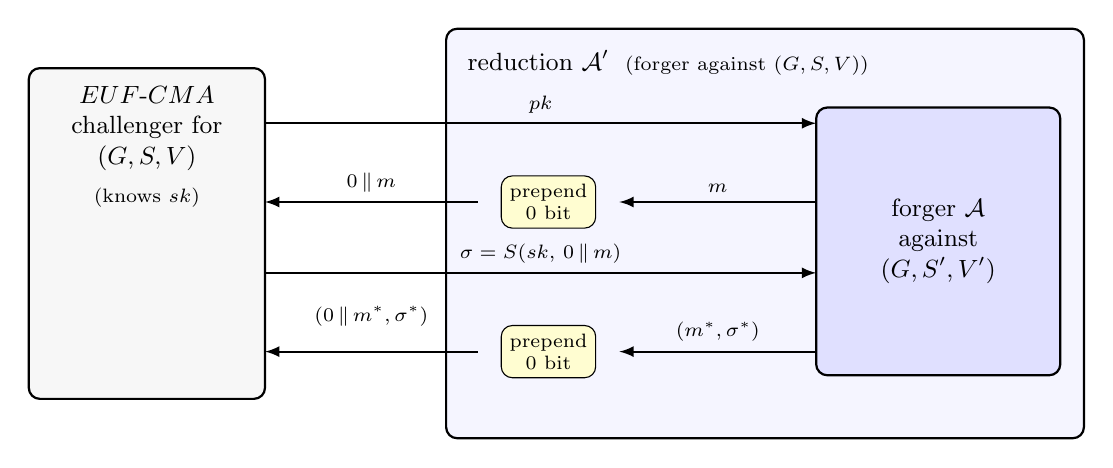
\begin{tikzpicture}[font=\small, >=latex,
   wire/.style={->, thick},
   trans/.style={draw, rounded corners, fill=yellow!18, inner sep=3pt, font=\scriptsize, align=center}]

% ---- Challenger (base scheme) ----
\draw[thick, rounded corners, fill=black!3] (0,0) rectangle (3,4.2);
\node[align=center] at (1.5,3.2)
  {$\game{\algo{EUF\text{-}CMA}}{}$\\ challenger for\\ $(G,S,V)$\\[3pt] \scriptsize(knows $sk$)};

% ---- Outer reduction box A' ----
\draw[thick, rounded corners, fill=blue!4] (5.3,-0.5) rectangle (13.4,4.7);
\node[anchor=north west] at (5.45,4.55) {reduction $\adv'$ \;\scriptsize(forger against $(G,S,V)$)};

% ---- Inner forger box A ----
\draw[thick, rounded corners, fill=blue!12] (10,0.3) rectangle (13.1,3.7);
\node[align=center] at (11.55,2.0) {forger $\adv$\\ against\\ $(G,S',V')$};

% ---- pk wire (challenger -> A) ----
\draw[wire] (3,3.5) -- (10,3.5);
\node[font=\scriptsize, above] at (6.5,3.5) {$pk$};

% ---- oracle query (A -> challenger), translated ----
\draw[wire] (10,2.5) -- (7.5,2.5);
\draw[wire] (5.7,2.5) -- (3,2.5);
\node[font=\scriptsize, above] at (8.75,2.5) {$m$};
\node[trans] at (6.6,2.5) {prepend\\ $0$ bit};
\node[font=\scriptsize, above] at (4.35,2.5) {$0\,\|\,m$};

% ---- oracle response (challenger -> A), unchanged ----
\draw[wire] (3,1.6) -- (10,1.6);
\node[font=\scriptsize, above] at (6.5,1.6) {$\sigma = S(sk,\,0\,\|\,m)$};

% ---- forgery output (A -> challenger), translated ----
\draw[wire] (10,0.6) -- (7.5,0.6);
\draw[wire] (5.7,0.6) -- (3,0.6);
\node[font=\scriptsize, above] at (8.75,0.6) {$(m^*,\sigma^*)$};
\node[trans] at (6.6,0.6) {prepend\\ $0$ bit};
\node[font=\scriptsize, above] at (4.35,0.8) {$(0\,\|\,m^*,\sigma^*)$};

\end{tikzpicture}
\caption{The security reduction drawn in the standard ``box-within-a-box'' style.\label{fig:reduction}}
\end{figure}

Now we check that $\adv'$ wins its game exactly when $\adv$ wins. First, whenever $\adv$'s forgery verifies, so does ours, because $V'(pk, m^*, \sigma^*) = V(pk, 0\,\|\,m^*, \sigma^*)$ by definition. Second, we must confirm the forgery is on a fresh message, i.e., that $0\,\|\,m^*$ was never sent to our own oracle. The only messages we ever sent to our oracle were of the form $0\,\|\,m$ for messages $m$ that $\adv$ queried, and $\adv$ winning means $m^*$ differs from all of those $m$; hence $0\,\|\,m^*$ differs from every message we queried, so it is fresh. Therefore $\adv'$ wins precisely when $\adv$ does, giving $\advantage{EUF\text{-}CMA}{\adv'} = \advantage{EUF\text{-}CMA}{\adv}$, which is non-negligible. Finally, $\adv'$ is PPT because it just runs $\adv$ (which is PPT) plus one extra bit of bookkeeping per oracle query. This contradicts the assumed security of $(G,S,V)$, completing the reduction.\\

It is worth naming the moving parts, since every EUF-CMA security proof you write will have them: (i) identify which scheme's security is the assumption and which is the conclusion; (ii) use the forger for the conclusion-scheme as a subroutine; (iii) \emph{simulate its signing oracle} using your own oracle; (iv) \emph{translate its forgery} into a forgery for your scheme; and (v) verify that your translated forgery is both valid \emph{and} on a message you never queried.\\

\textbf{Example: breaking a scheme.} Not every transformation preserves security, and showing that a scheme is \emph{insecure} is usually easier: we only have to exhibit a single PPT adversary with non-negligible advantage. Consider the scheme $(G, S', V')$ on message space $\{0,1\}^\lambda$ (with $\lambda \ge 2$) that signs the message after \emph{deleting its last bit}: writing $m = b_1 b_2\cdots b_\lambda$, $$S'(sk, m) = S(sk, b_1\cdots b_{\lambda-1}), \qquad V'(pk, m, \sigma) = V(pk, b_1\cdots b_{\lambda-1}, \sigma).$$ The problem is that any two messages differing only in their last bit receive the very same signature, which lets us forge after a single query (see Figure \ref{fig:attack}):
\begin{enumerate}[(1)]
\item Query the signing oracle on $m = 0^\lambda$ (the all-zeros message), receiving $\sigma = S'(sk, 0^\lambda) = S(sk, 0^{\lambda-1})$.
\item Output the forgery $(m^*, \sigma^*) = (0^{\lambda-1}1,\ \sigma)$.
\end{enumerate}

\begin{figure}[tbhp]
\centering
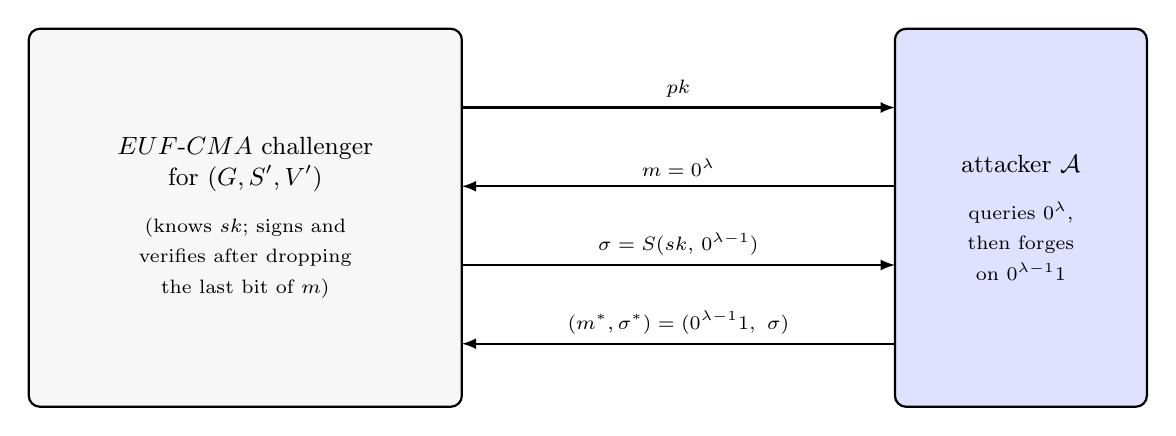
\begin{tikzpicture}[font=\small, >=latex,
   wire/.style={->, thick}]

% ---- Challenger (modified, insecure scheme) ----
\draw[thick, rounded corners, fill=black!3] (0,-0.3) rectangle (5.5,4.5);
\node[align=center] at (2.75,2.1)
  {$\game{\algo{EUF\text{-}CMA}}{}$ challenger\\ for $(G,S',V')$\\[6pt] \scriptsize(knows $sk$; signs and\\ \scriptsize verifies after dropping\\ \scriptsize the last bit of $m$)};

% ---- Attacker ----
\draw[thick, rounded corners, fill=blue!12] (11,-0.3) rectangle (14.2,4.5);
\node[align=center] at (12.6,2.1) {attacker $\adv$\\[6pt] \scriptsize queries $0^\lambda$,\\ \scriptsize then forges\\ \scriptsize on $0^{\lambda-1}1$};

% ---- pk wire (challenger -> attacker) ----
\draw[wire] (5.5,3.5) -- (11,3.5);
\node[font=\scriptsize, above] at (8.25,3.5) {$pk$};

% ---- query (attacker -> challenger) ----
\draw[wire] (11,2.5) -- (5.5,2.5);
\node[font=\scriptsize, above] at (8.25,2.5) {$m = 0^\lambda$};

% ---- response (challenger -> attacker) ----
\draw[wire] (5.5,1.5) -- (11,1.5);
\node[font=\scriptsize, above] at (8.25,1.5) {$\sigma = S(sk,\,0^{\lambda-1})$};

% ---- forgery (attacker -> challenger) ----
\draw[wire] (11,0.5) -- (5.5,0.5);
\node[font=\scriptsize, above] at (8.25,0.5) {$(m^*,\sigma^*) = (0^{\lambda-1}1,\ \sigma)$};

\end{tikzpicture}
\caption{The forgery attack of the previous example. Unlike Figure \ref{fig:reduction}, this is not a reduction: the attacker $\adv$ is a single program playing the EUF-CMA game directly against the modified scheme $(G,S',V')$, whose signing oracle and verifier both drop the last bit of a message.\label{fig:attack}}
\end{figure}

The message $m^* = 0^{\lambda-1}1$ was never queried (it differs from $0^\lambda$ in the last bit), so it is fresh, yet $V'(pk, m^*, \sigma) = V(pk, 0^{\lambda-1}, \sigma) = \text{true}$ because $\sigma$ is a genuine base-scheme signature on $0^{\lambda-1}$. This adversary wins with probability $1$, so $\advantage{EUF\text{-}CMA}{\adv} = 1$, which is certainly not negligible, and hence $(G, S', V')$ is not EUF-CMA secure. Notice the shape of an attack: choose specific oracle queries, output a specific forgery, and argue both that it verifies and that its message is fresh.\\

Now you are ready to try both directions yourself.

\begin{exercise}
Let $(G, S, V)$ be a secure signature scheme with the message space $\{0,1\}^\lambda$. Let $\hat{G}$ be a new key generation function that simply calls $G$ twice and returns a pair of secret keys, $(sk_0, sk_1)$, and the corresponding pair of public keys, $(pk_0, pk_1)$. Which of the following signature schemes, $(\hat{G}, \hat{S}, \hat{V})$, are secure? Show an attack or prove security (by reduction).
\begin{enumerate}[(a)]
\item Prove that ``Sign halves'' is \textbf{not} secure: $$\hat{S}((sk_0, sk_1), (m_L, m_R)) = (S(sk_0, m_L), S(sk_1, m_R)),$$ $$\hat{V}((pk_0, pk_1), (m_L, m_R), (\sigma_0, \sigma_1)) = V(pk_0, m_L, \sigma_0)\wedge V(pk_1, m_R, \sigma_1).$$
\item Show that ``Sign with randomness'' is \textbf{not} secure: $$\hat{S}(sk_0, m) = [\text{choose random }r\in\{0,1\}^\lambda; \text{output }(r, S(sk_0, m\oplus r), S(sk_0, r))],$$ $$\hat{V}(pk_0, m, (r, \sigma_0, \sigma_1)) = V(pk_0, m\oplus r, \sigma_0)\wedge V(pk_0, r, \sigma_1).$$
\item Prove that ``Accept one valid'' is secure: $$\hat{S}((sk_0, sk_1), m) = (S(sk_0, m), S(sk_1, m)),$$ $$\hat{V}((pk_0, pk_1), m, (\sigma_0, \sigma_1)) = V(pk_0, m, \sigma_0)\vee V(pk_1, m, \sigma_1).$$ (Hint: Consider using that $\pr{\sigma_0\text{ or }\sigma_1\text{ is valid}} \leq \pr{\sigma_0\text{ valid}} + \pr{\sigma_1\text{ valid}}$ from Exercise 4 of last week).
\end{enumerate}
\end{exercise}

Now we are almost ready to see the Fiat-Shamir Transform (next week), which turns secure identification protocols into secure digitial signature schemes. We will use the Fiat-Shamir Transform to prove the security of the Schnorr signature soon. The only ingredient missing is the Random Oracle Model (ROM), which is how we model our hash functions to make proofs more practical:

\begin{reading}
Read about the Random Oracle Model in:\\
Jonathan Katz and Yehuda Lindell - Introduction to Modern Cryptography - pages 187-191.
\end{reading}

Pieter recorded the following video further discussing the ROM: \url{https://www.youtube.com/watch?v=ITxL4bOkOy0}\\

One strange but important feature of the ROM discussed in the section ``Definitions and Proofs in the ROM'' is that during a reduction, adversaries $\adv$ must ``report'' all of their oracle queries to the adversary $\adv'$ that is using $\adv$ as a subroutine, and additionally $\adv'$ may adaptively control the response that $\adv$ gets to these queries so long as $\adv$ cannot distinguish what they receive from a regular random oracle. This kind of reporting feature is also key to other models we will discuss in the future.\\

Next week, we will use the Random Oracle Model (ROM) to construct the Fiat-Shamir transform, and then we will dive straight into proving that the Schnorr digital signature is secure!

%In the following reading, I personally think their introduction of $(I, \text{st})$ in the definition of an identification protocol is a little bit confusing. I encourage you to think of the initial message, $I$, as just some random ``public key'', whose ``private key'', $\text{st}$, will be used in the prover's final response to ensure that they are not leaking their usual private key. Additionally, I think they could mention sooner than they do that step 1 of Algorithm $\adv$ in the proof of Theorem 13.10 is literally just guessing which of the queries that $\adv'$ makes to the random oracle contains the message that $\adv'$ is trying to create a forgery for, and acting accordingly after making this guess. This makes it very unlikely ($\frac{1}{q}$ chance the guess was correct) that Algorithm $\adv$ succeeds, even if $\adv'$ \emph{always} succeeds. However, because there is a polynomial bound on the number of oracle queries $\adv'$ makes, even if $\adv$ is worse than $\adv'$ we still get that $\adv$ has a non-negligible success probability if $\adv'$ does ($\frac{1}{q}$ is non-negligible).

%\begin{reading}
%Read about the Fiat-Shamir Transform in:\\
%Jonathan Katz and Yehuda Lindell - Introduction to Modern Cryptography - Section 13.5.1.
%\end{reading}

%Finally, we are ready to read a proof of the security of the Schnorr signature in the ROM! The final part of the proof where they discuss probabilities is a little bit tricky, but try to get at least a high-level understanding and we can discuss this in detail together.

%\begin{reading}
%Read about the Schnorr signature's security in:\\
%Jonathan Katz and Yehuda Lindell - Introduction to Modern Cryptography - Section 13.5.2.
%\end{reading}

\end{document}